\graphicspath{{Chapters/Chapter_ml-dataruns/}}

\chapter{Creating a randomized  dataset for machine learning tasks}
\label{ch:ml-dataruns}

\section{Goal and introduction}

The goal of collecting this dataset was to maximize the diversity of data coming from the LAPD. Previous datasets -- even one made of 29 million passively-collected shots over three years -- did not contain sufficient diversity to conduct an interesting ML study. In particular, the data must be sufficiently diverse to allow an optimization study without the need to collect more data. In addition, many diagnostics were recorded so that the signals could be correlated on the same shot, either in the machine learning model itself or as a preprocessing step. This chapter describes the process of collecting these data, example signals, and biases within the dataset. All of the data from this campaign (several terabytes) is available upon request. 

The LAPD has many experimental control parameters for various physics studies. While the device can accommodate various insertable components, this dataset focuses on the parameters fundamental to the operation of the main cathode. Specifically, half way between the cathode and anode are three gas puff valves: East, West, and top. The aperture, duration, and triggering of these valves has a large impact on plasma formation. A static gas fill system also exists but it is not used. The cathode-anode voltage (and consequently, discharge power) strongly influences plasma density and temperature downstream of the source. Additionally, the magnetic field configuration substantially shapes the plasma column. One crucial variable not considered in this dataset is the cathode temperature, as its adjustment and equilibration requires many hours, limiting dataset diversity. This combination of diagnostic coverage, high repetition rate, and extensive configurability renders the LAPD particularly suitable for machine learning studies. 

\section{Configuration of the LAPD}

Data collection was conducted in two campaigns separated by 14 months. The initial run set is designated as \texttt{DR1} and the subsequent run set as \texttt{DR2}. These run sets are further broken down into \emph{dataruns} which are series of discharges (``shots'') with identical operational machine parameters. A total of 67 dataruns were collected over both campaigns. These two datarun sets had significant intrinsic differences: \texttt{DR1} had two turbomolecular pumps offline, leading to much higher background pressures. Furthermore, the cathode condition in terms of emissivity or asymmetries is unquantified, so there may be intrinsic differences in the plasma produced regardless of machine configuration. 

The LAPD control parameters varied in this dataset were the source field, mirror field, midplane field, gas puff valve voltage, gas puff duration, and discharge voltage. The magnetic field regions are labeled in fig. \ref{fig:ml-lapd-diagnostics} and effectively control the width of the plasma relative to the cathode in their respective regions. The gas puff voltage governs gas flow rate into the chamber, though this relationship is not yet quantified, and the gas puff duration defines the piezo valve activation period. For \texttt{DR1}, the discharge voltage is applied across the cathode and anode at the same time as the gas puff, but for \texttt{DR2} applied 10 ms after gas puff initiation. This difference between runs was not known at experiment time. While discharge voltage correlates to discharge current (and thus power), the current depends on the machine configuration and downstream conditions and cannot be predetermined.

These machine parameters -- with the exception of gas puff duration -- were randomly sampled via Latin-hypercube sampling (LHS) for 44 of the dataruns. LHS is a pseudorandom sampler that guarantees that each machine setting is set at least once. An example of LHS vs random sampling can be seen in fig. \ref{fig:lhs-vs-random}. It is possible for random sampling to miss certain machine settings, or entire portions of configuration space altogether. This fact is particularly important when the number of samples is small, such as in this case with 44 samples. Data were then collected with these settings. Gas puff duration was reduced for the last seven runs to 20, 10, or 5 ms (see fig. \ref{fig:PP1_time-series-example} for timings relative to $I_\text{sat}$ signals). The breakdown of each setting in the dataset is given in appendix \ref{sec:app_bias}, Table \ref{tab:data_frac}. The top gas puff valve was used for only the first nine dataruns of \texttt{DR2} because of equipment issues. 23 of the dataruns in the dataset are not random: they were chosen to be similar to common machine configurations used in more conventional studies, usually using flat fields (or different cathode fields) around 1 kG. These data were taken while other diagnostics were being configured.

\begin{figure}
	\centering
	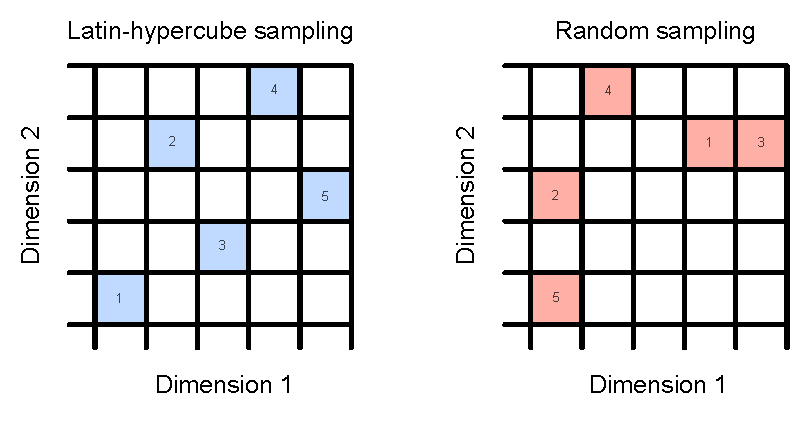
\includegraphics[width=350pt]{figures/lhs.pdf}
	\caption[A demonstration of Latin-hypercube sampling vs random sampling]{\label{fig:lhs-vs-random}An example of Latin Hypercube Sampling compared to a potential random sample of five points. LHS hits all rows and columns, but random sampling may leave some sections of parameter unsampled space altogether.}
\end{figure}

$I_\text{sat}$ and other probe-based measurements were acquired along y=0 lines (51 dataruns total) or x-y grids (16 dataruns total) with spatial resolutions varying between 1.5 to 2 cm. The fixed axial locations of the probes were 895 cm and 831 in \texttt{DR1} and 1150, 1022, 863, and 639 cm for \texttt{DR2} (Fig. \ref{fig:LAPD_coords}). Six shots were recorded at each position except for the first four dataruns in \texttt{DR1} with five shots each.

\section{Signals collected}

\texttt{DR1} and \texttt{DR2} had considerable overlap in diagnostics recorded, with some minor differences. A summary of the diagnostics and their locations on the LAPD can be seen in fig. \ref{fig:ml-lapd-diagnostics}. Some of the raw diagnostics signals and machine state information (MSI) can be seen in fig. \ref{fig:example-diagnostics-msi}. Some dataruns may not contain all diagnostics, as some data were collected while other diagnostics were being set up. The diagnostics and machine state information (MSI) recorded for this dataset are the following:
\begin{itemize}
	\item \textbf{\texttt{DR1} probes}: three probes were inserted into the LAPD. One had Langmuir sweeps, another ``flux probe'' had $I_\text{sat}$ and two floating potential (V$_\text{f}$) tips, and the last ``triple probe'' had $I_\text{sat}$, V$_\text{f}$ and electron temperature ($T_e$). These signals were digitized at 6.25 MHz (100 MHz, 16 sample average).
	\item \textbf{\texttt{DR2} probes}: four probes were inserted, namely a flux probe, triple probe, Langmuir sweeps with $I_\text{sat}$ on a separate tip, and another flux probe. These signals were digitized at 6.25 MHz (100 MHz, 16 sample average).
	\item \textbf{Diodes}: five diodes, axially distributed, were recorded as well. The one closest to the cathode had a He-II line filter. The diodes were uncalibrated, have a nonlinear response, and are sensitive beyond the visible spectrum. These diodes were a part of the MSI system and were recorded at 25 kHz. Each diode (besides the one with the He-II filter) had 8 layers of 1-stop (50\% transmission) neutral density filter in front of the diode.
	\item \textbf{Interferometer}: signals from the 288 GHz heterodyne interferometer were recorded on an oscilloscope at 10 MHz, which was then downsampled to 100 kHz before analysis so that the processing computer could keep pace.
	\item \textbf{Thomson scattering}: a single point was measured on-axis at port 32, triggered at 8 ms into the plasma for \texttt{DR1} or 12 ms for \texttt{DR2}. Periodically the collection optics were scanned to maximize the light collected during both run sets.
	\item \textbf{Spectrometer}: an Ocean Optics HR4000 spectrometer recorded spectra integrated over the duration of the shot. The spectrometer has a very narrow slit, leading to good spectral resolution but requiring many shots for a clean spectrum.
	\item \textbf{Monochromator (\texttt{DR2} only}): three Helium neutral lines were recorded, namely 587, 667, and 707 nm, using an oscilloscope sampling at 1 MHz.
	\item \textbf{Diamagnetic loop}: the loop sits between ports 34 and 35 and consists of one large loop and two smaller concentric loops equaling the area of the large one. These signals were digitized using an oscilloscope at 500 kHz, but are strongly influenced by magnet power supply noise making analysis difficult.
	\item \textbf{Fast framing camera}: a Phantom v7.3 fast framing camera recorded plasma dynamics from the end of the machine, pointing towards the cathode. The images are monochrome, 14 bit, 14 $\mu$s exposure, $256\times256$ pixels, and 2,500 fps using a 105 mm lens. The camera is capable of 36,697 fps at that resolution, but a lower one was used to lessen file transfer times and storage requirements.
	\item \textbf{Discharge current and voltage}: as part of the MSI system, time series of discharge current and voltage are recorded at 25 kHz.
	\item \textbf{Magnetic field profiles}: theoretical on-axis magnetic field values are calculated using the magnet power supplies. Both are recorded as part of the MSI. For the work here, we simply use the programmed field values for the cathode, mirror, and midplane regions. Occasionally the calculated field would be incorrect since the power supply currents for the cathode are set manually, which is the case in some dataruns here, but the profiles are unused in these studies so it isn't an issue.
	\item \textbf{Pressures}: total pressure and pressure breakdown by atomic mass unit are recorded by an ion gauge and RGA, respectively. The RGA takes approximately two minutes to complete a scan but the data should be reasonably accurate given the slow time-evolution of pressure.
\end{itemize}

\begin{figure}
	\centering
	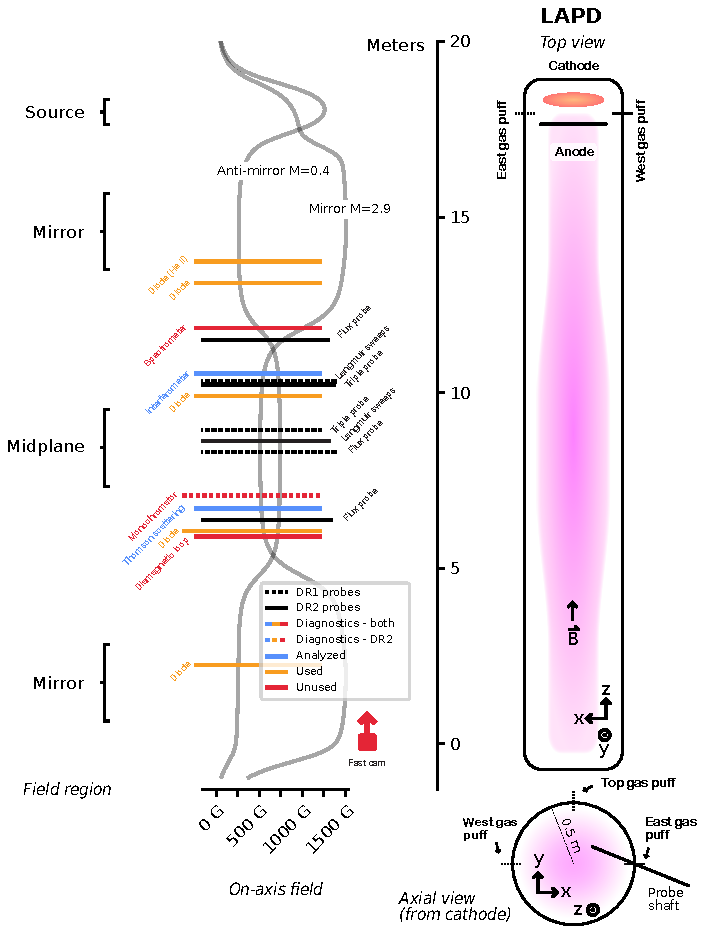
\includegraphics[width=440pt]{figures/lapd-diagnostics.pdf}
	\caption[LAPD configuration and diagnostics for the ML datarun]{\label{fig:ml-lapd-diagnostics}Diagnostics and example field configurations for \texttt{DR1} and \texttt{DR2}}
\end{figure}

\begin{figure}
	\centering
	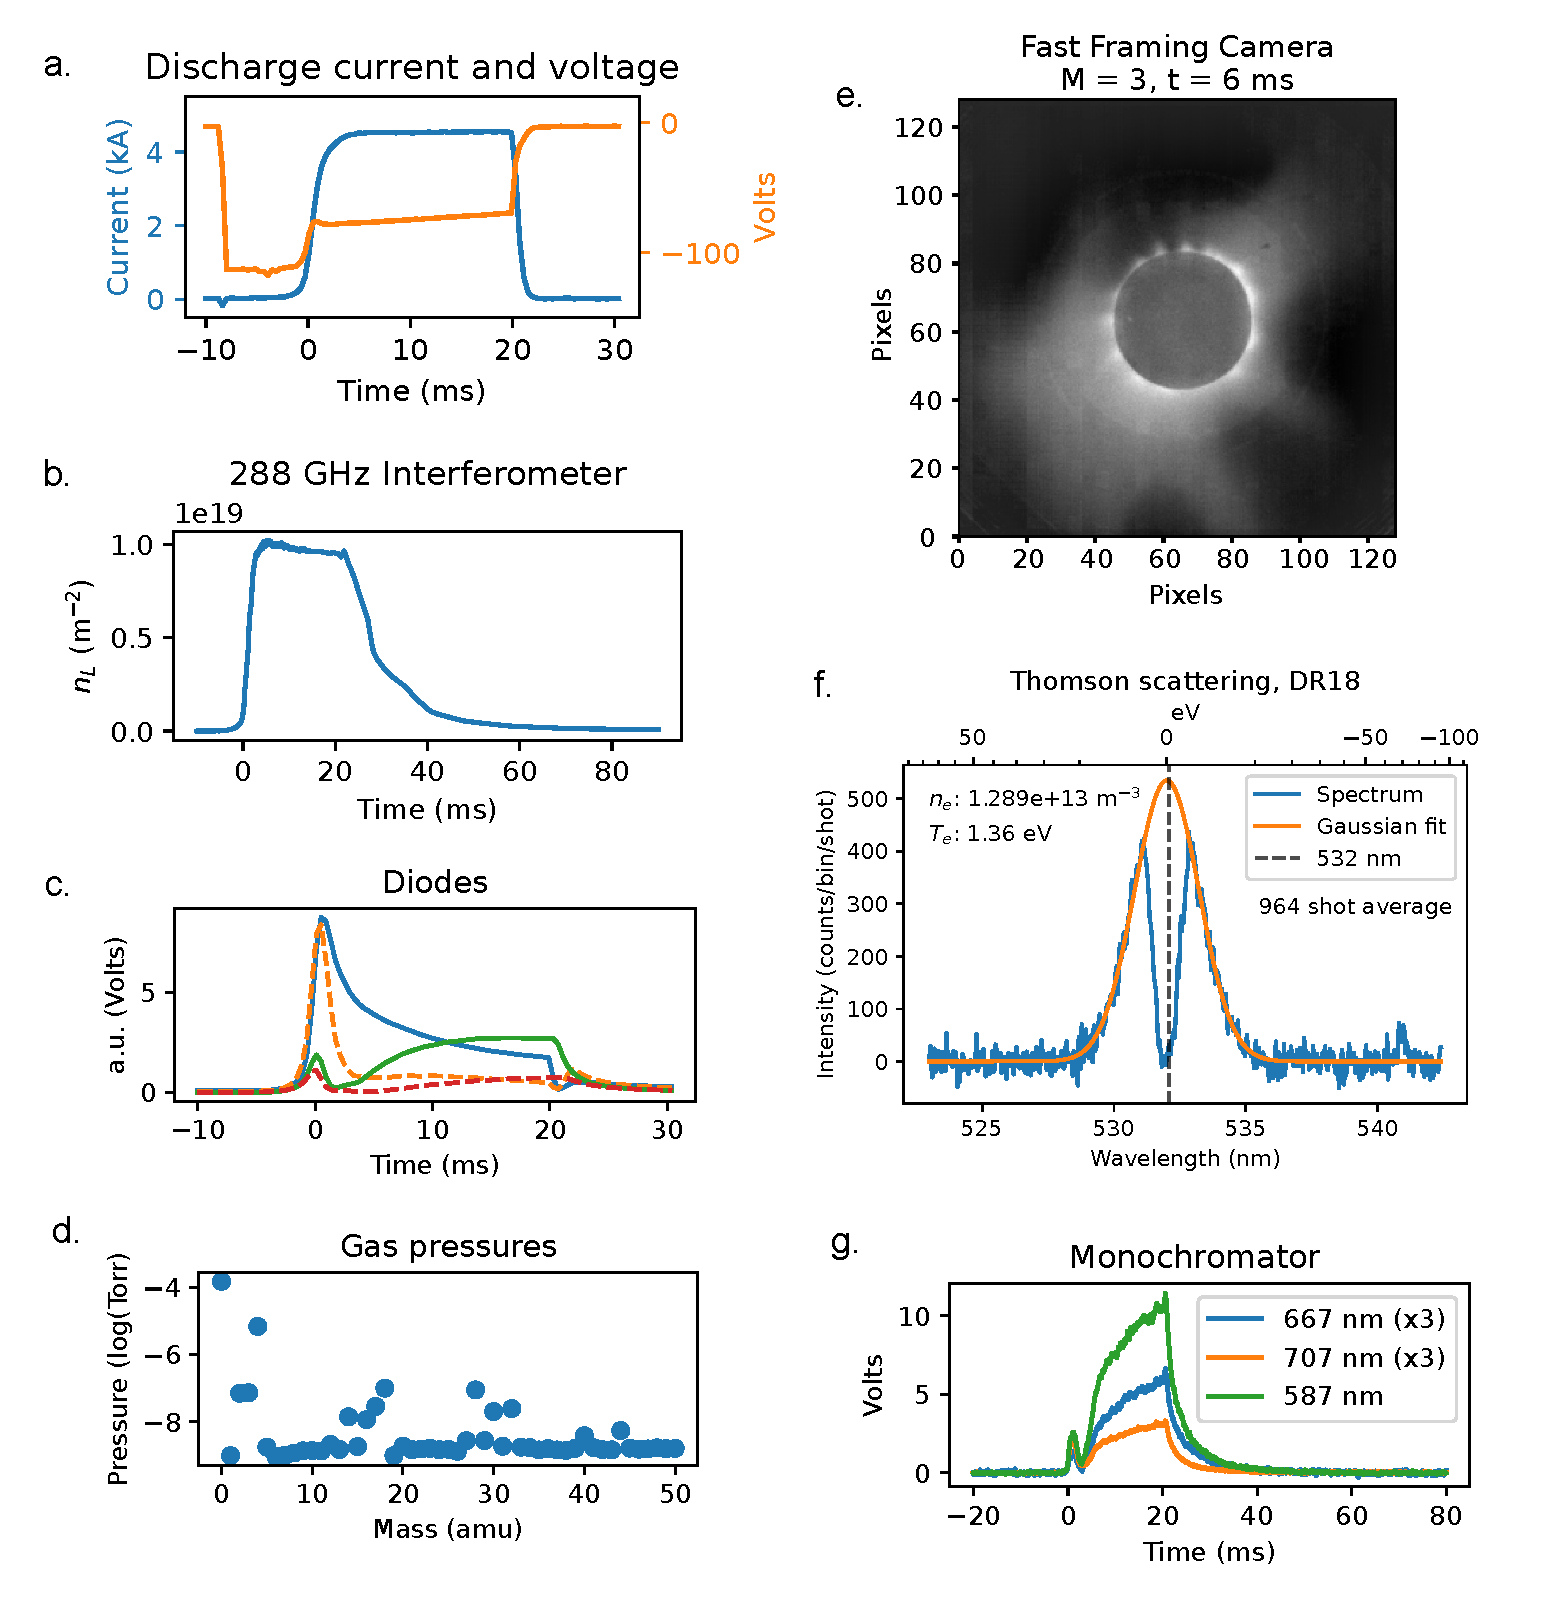
\includegraphics[width=450pt]{figures/diagnostics-examples.pdf}
	\caption[Example machine state information and diagnostic signals]{\label{fig:example-diagnostics-msi}Example diagnostic signals and machine state information from a variety of discharges.}
\end{figure}

Of the probes, only $I_\text{sat}$ was analyzed and used. The interferometer and Thomson scattering signals were also analyzed. The diode signals were unanalyzed but used in a downstream machine learning study. The spectrometer, monochromator, and diamagnetic loop remain unanalyzed and unused, but the raw signals could be useful for ML studies as will be shown with the diode signals (see chapter \ref{ch:ebm}). The fast framing camera was useful for checking probe alignment and visualizing plasma structure, but it was otherwise not used or analyzed for the downstream ML studies.

\section{Data cleaning}

$I_\text{sat}$ measurements in \texttt{DR1} that saturated either the isolation amplifier or digitizer are excluded from the dataset. Only 484 shots were removed out of $\approx$132,000, so the impact on the aggregate dataset is minimal. This signal saturation was detected while data were being taken and was corrected quickly.

Interferometer skips were occasionally seen, likely caused by large $\delta n / n$ structures combined with downsampling before conversion of the signal into a density measurement. Attempts were made to unwrap these skipping traces (see fig. \ref{fig:ifo-skip}) but without much success, so these shots were cut from the dataset.

\begin{figure}
	\centering
	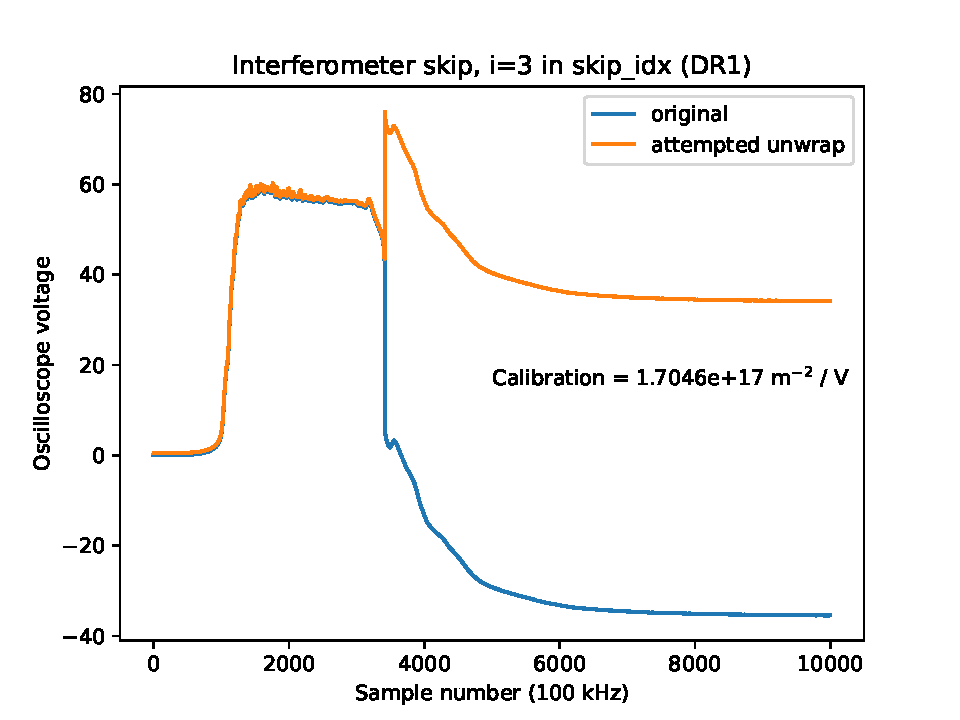
\includegraphics[width=300pt]{figures/ifo_skip_example.pdf}
	\caption[Example interferometer skips]{\label{fig:ifo-skip} An example of the interferometer skip (blue) and the attempted unwrap (orange).}
\end{figure}

The Thomson scattering (TS) diagnostic was available only for dataruns 8 and onwards in \texttt{DR1}. The TS image data did not have timestamps recorded, so a rough estimate was used based on filename and last saved time. Uncertainty in time is tolerable because conditions were identical to datarun shots for a few minutes before and after the dataruns. Fits were taken of the average over the entire datarun; each shot in a datarun has the same recorded TS temperature and density. 
Dataruns were removed if the error on the density, measured by the square root of the covariance of the fit amplitude, was greater than 50\%. Fits above that error threshold were largely unusable. A couple of dataruns looked like pure noise even when averaged over several hundred shots, but were not caught by this broad criterion. 24 dataruns remained out of 30.
In some runs there was high-pixel-frequency noise at 128 and 256 (every 4th and 2nd pixel, respectively). The fitting routine is typically insensitive to this cleaning process, but significant differences can be seen in particularly low-density plasmas where the photon counts are low. An example of this process can be seen in fig. \ref{fig:TS_fit-and-FFT}.

\begin{figure}
	\centering
	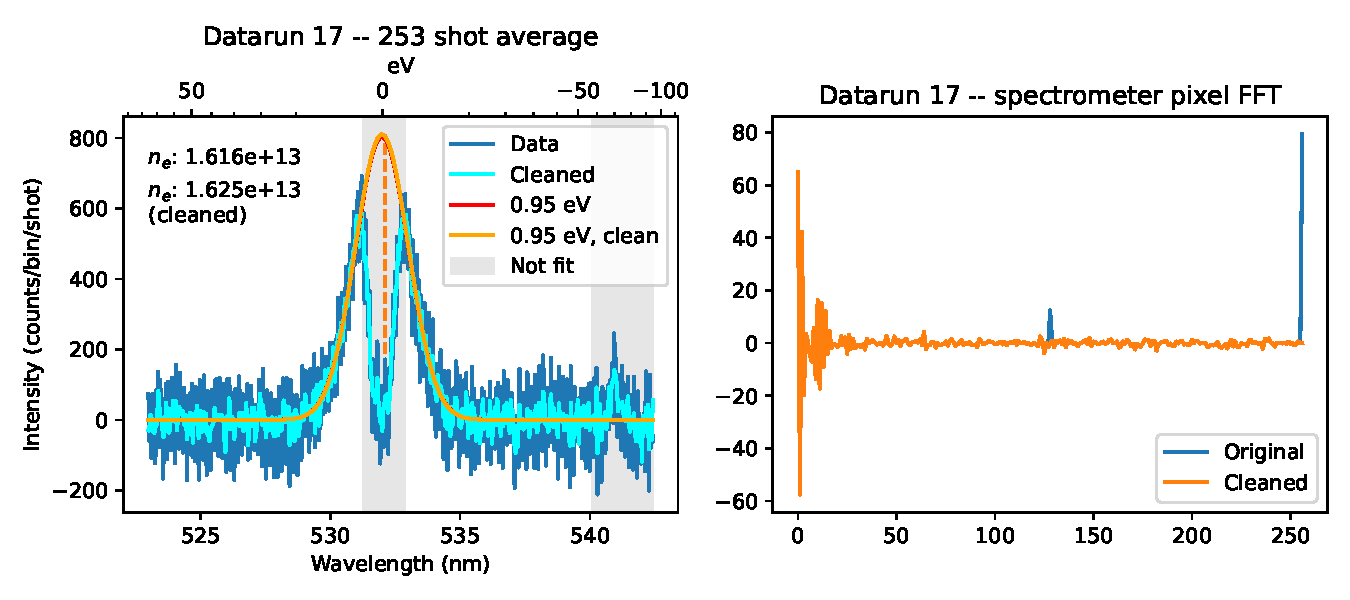
\includegraphics[width=\linewidth]{figures/TS_fit-and-FFT.pdf}
	\caption[Cleaning Thomson scattering spectra]{\label{fig:TS_fit-and-FFT} The Gaussian fit to the Thomson scattering spectrum before and after crude FFT filtering. The shaded gray region is excluded from the fitting process because they contain the region of the notch filter (the region about 532 nm) and a He-II (ion) line ($\approx 541$ nm).}
\end{figure}


\section{Data bias \label{sec:app_bias}}

Data bias and imbalance in the training set can be exacerbated by the train-test split. For the nominal test set, 8 out of the 67 dataruns were hand-picked for diversity and held out from the training set. Leaving out entire dataruns -- not just shots -- is important in order to estimate model performance on new, unseen discharges in new configurations. Four dataruns from each run set were left out: for \texttt{DR1} 08, 15, 23, and 33; for \texttt{DR2}, 02, 10, 19, and 31. As will be demonstrated in chapter \ref{ch:isat-predict}, this test set appears to characterize the model performance on held out data fairly well.

The dataset predominantly contains gas puff durations of 38 ms. Only six runs in the training set have gas puff durations less than 38 ms: three have 5 ms and three have 10 ms, each having mirror ratios 1, 3, and 6 but otherwise identical configurations in an attempt to see mirror-related interchange instabilities in higher-temperature, lower-collisionality regimes. The 20 ms gas puff duration case is in the test set (\texttt{DR2} 31). This sampling bias towards the 38 ms gas puff duration suggests poor model performance is to be expected in shorter gas puff regimes. The top gas puff valve was operational for only the first nine runs of \texttt{DR2}.

\begin{figure*}
	\centering
	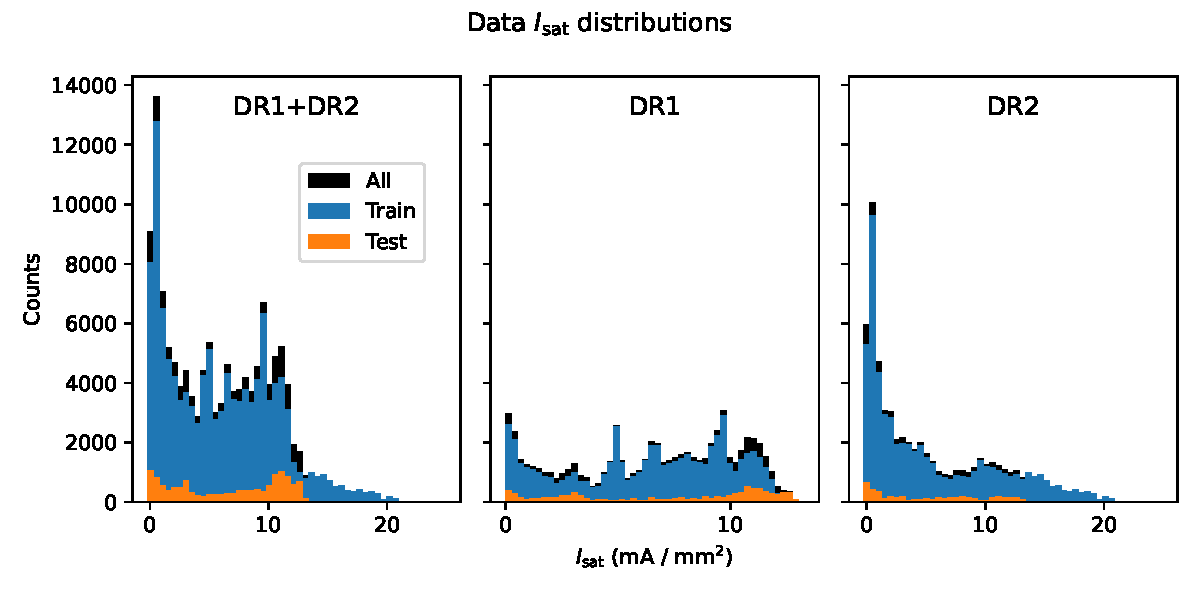
\includegraphics[width=\linewidth]{figures/PP1_02_isat_distribution.pdf}
	\caption[Time-averaged $I_\text{sat}$ distribution over shots]{\label{fig:PP1_02_isat_distribution}Distribution of $I_\text{sat}$ signals when averaged from 10 to 20 ms. \texttt{DR1} appears to have a more uniform distribution than \texttt{DR2} does. Combining the two datasets results in many $I_\text{sat}$ examples near 0 mA/mm$^2$ and a sharp decrease in number of examples above 10 mA/mm$^2$. From these histograms we expect our model to be biased towards fitting lower $I_\text{sat}$ values better, and to perform poorly in cases with very high $I_\text{sat}$ values.}
\end{figure*}

Despite the best efforts to randomize the machine configuration, imbalance in the dataset will be present because of the relatively small amount of samples for the given actuator space. The distribution of $I_\text{sat}$ signals, averaged from 10 to 20 ms, can be seen in Fig. \ref{fig:PP1_02_isat_distribution}. The $I_\text{sat}$ distribution is clearly different for \texttt{DR1} and \texttt{DR2}, with \texttt{DR1} having a much flatter distribution. These distributions imply that if the model is constrained to sample from \texttt{DR2} via the run set flag, then the model is expected to predict a lower $I_\text{sat}$ value in general. When predicting from the model in general, performance will likely be worse for $I_\text{sat}$ values $\gtrsim 11$ mA/mm$^2$. The time-averaged $I_\text{sat}$ distribution is dissimilar between \texttt{DR1} and \texttt{DR2}: \texttt{DR1} appears to have a more uniform distribution. Combining the two datasets results in many $I_\text{sat}$ examples less than 2 mA/mm$^2$ and a sharp decrease in number of examples above 10 mA/mm$^2$. Thus, we expect the model to perform better for smaller $I_\text{sat}$ values than larger ones. 

The mix of different probe movements also leads to some imbalance in the dataset. The distribution of probe positions can be seen in fig. \ref{fig:PP1_02_x_distribution}. Notably, samples appear to drop off beyond +25 cm and -15 cm. Measurements over an x-y plane, constituting $\approx 64\%$ of all shots, are predominantly acquired overnight for maximal machine utilization. These longer dataruns lead to particular machine configurations being overrepresented in the dataset. 

\begin{figure}
	\centering
	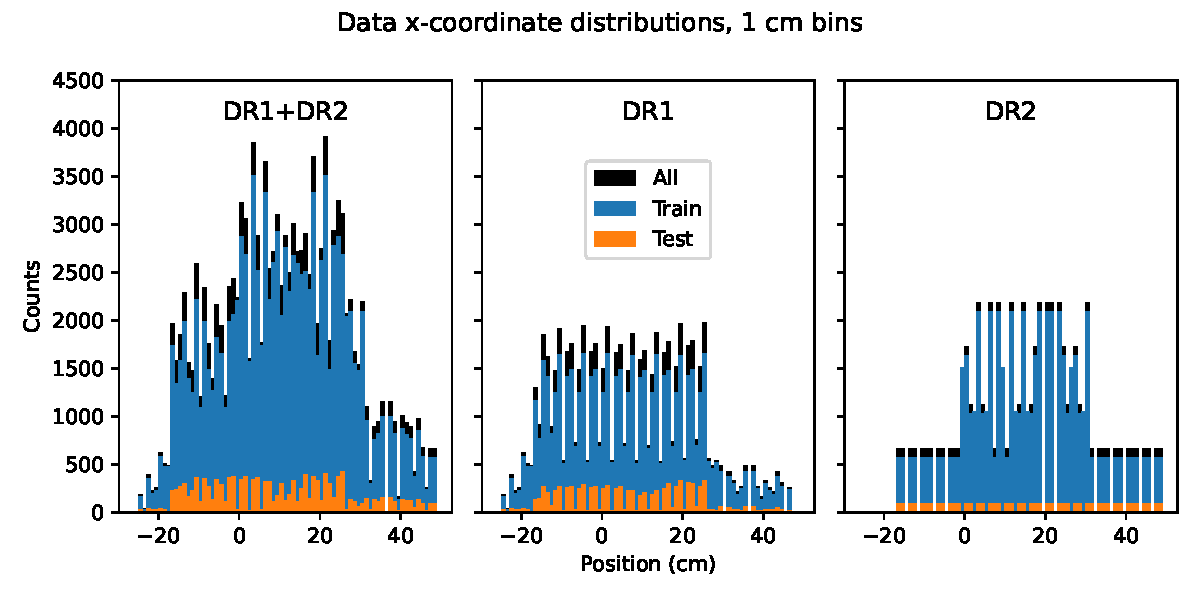
\includegraphics[width=\linewidth]{figures/PP1_02_x_distribution.pdf}
	\caption[Distribution of probe x-coordinates in the dataset]{\label{fig:PP1_02_x_distribution}Distribution of the x-coordinate in the profiles. The increase in data points between roughly x $\approx 0$ to 30 cm is from planes instead of lines. Based on this distribution, the performance of the model is expected to be biased towards this central area.}
\end{figure}

\begin{table*}
\small
	\centering
	\caption{Data breakdown by class and dataset (percent)}
	\label{tab:data_frac}
	\begin{tabular}{lrrr|lrrr|lrrr}
		\multicolumn{4}{c|}{B source (G)} & \multicolumn{4}{c|}{B mirror (G)} & \multicolumn{4}{c}{B midplane (G)}\\
		\hline \hline
		& Train & Test & All && Train & Test & All && Train & Test & All \\
%		\cline{2-4} \cline{6-8} \cline{10-12}
		500 & 4.77 & 0 & 4.29 & 250 & 4.30 & 8.41 & 4.72 & 250 & 8.25 & 21.01 & 9.55 \\
		750 & 3.34 & 12.61 & 4.29 & 500 & 30.49 & 8.41 & 28.23 & 500 & 43.80 & 8.41 & 40.19 \\
		1000 & 43.13 & 78.99 & 46.78 & 750 & 6.68 & 16.81 & 7.72 & 750 & 6.62 & 52.19 & 11.27 \\
		1250 & 12.59 & 0 & 11.30 & 1000 & 28.85 & 57.97 & 31.82 & 1000 & 26.36 & 5.78 & 24.26 \\
		1500 & 19.23 & 0 & 17.27 & 1250 & 3.34 & 4.20 & 3.43 & 1250 & 9.24 & 0 & 8.30 \\
		1750 & 1.91 & 0 & 1.71 & 1500 & 26.34 & 4.20 & 24.08 & 1500 & 5.73 & 12.61 & 6.43 \\
		2000 & 15.03 & 8.41 & 14.35 & & & & & & & & \\
		\\
		\multicolumn{4}{c|}{Gas puff voltage (V)} & \multicolumn{4}{c|}{Discharge voltage (V)} & \multicolumn{4}{c}{Axial probe position (cm)} \\
		\hline \hline
		70 & 12.11 & 16.81 & 12.59  & 70 & 12.22 & 8.41 & 11.83    & 639 & 12.48 & 8.41 & 12.06 \\
		75 & 6.68 & 0 & 6.00     & 80 & 5.25 & 0 & 4.72      & 828 & 17.07 & 36.28 & 19.03 \\
		80 & 11.46 & 8.41 & 11.15   & 90 & 2.86 & 8.41 & 3.43      & 859 & 12.48 & 8.41 & 12.06  \\
		82 & 41.49 & 57.97 & 43.17  & 100 & 3.34 & 8.41 & 3.86     & 895 & 33.01 & 30.10 & 32.71 \\
		85 & 14.13 & 0 & 12.69   & 110 & 8.77 & 0 & 7.87     & 1017 & 12.48 & 8.41 & 12.06 \\
		90 & 14.13 & 16.81 & 14.40  & 112 & 20.62 & 0 & 18.52   & 1145 & 12.48 & 8.41 & 12.06 \\
                      & & & & 120 & 3.82 & 8.41 & 4.29     &                       & & & \\
                      & & & & 130 & 0.95 & 0 & 0.86     &                       & & & \\
                      & & & & 140 & 2.86 & 8.41 & 3.43     &                       & & & \\
                      & & & & 150 & 39.30 & 57.97 & 41.20  &                       & & & \\
		\\
		\multicolumn{4}{c|}{Gas puff duration (ms)} & \multicolumn{4}{c}{Vertical probe position (cm)}\\
		\cline{0-7} \cline{0-7}
		$38$ & 94.27 & 91.59 & 94.00 & $\approx 0$ & 36.26 & 46.08 & 37.26 & \\
		$<38$ & 5.73 & 8.41 & 6.00    & $\neq 0$ & 63.74 & 53.92 & 62.74    & \\
		\multicolumn{12}{l}{}
	\end{tabular}
\end{table*}

The distribution of the selected machine settings for all the dataruns is enumerated in Table \ref{tab:data_frac}. Despite the randomization of the settings of 44 dataruns, the distribution is often uneven. The remaining 23 non-random dataruns also contribute to the imbalance. For example, a source field of 1 kG and discharge voltage of 112 show up disproportionately in the dataset because data were collected at those settings while other equipment was being adjusted or calibrated.

\section{Azimuthal asymmetry of probe data}

Examining the data, it appears that the y coordinate is not centered properly, possibly because the telescope used to align the probes is set incorrectly. Using profiles from planar data (see the ``before'' plot in fig. \ref{fig:y-alignment_before-after}), the y-coordinate was adjusted. The probes in DR1 were adjusted upward by 2 cm. For DR2, the y-coordinate was adjusted separately for each probe. Port 17 was adjusted 6 cm up, port 21 was adjusted 4 cm up, port 26 was adjusted 4.5 cm up, and port 33 was adjusted 3.35 cm up. This degree of error is consistent with a centering scope crosshair angle error, which would cause a larger absolute y-axis error closer to the cathode. An example of this y-axis error and the profile after shifting the coordinates can be seen in fig. \ref{fig:y-alignment_before-after}. It is likely that this y-axis offset applies to other probes in the plasma, not just probes with $I_\text{sat}$ tips. 

\begin{figure}
	\centering
	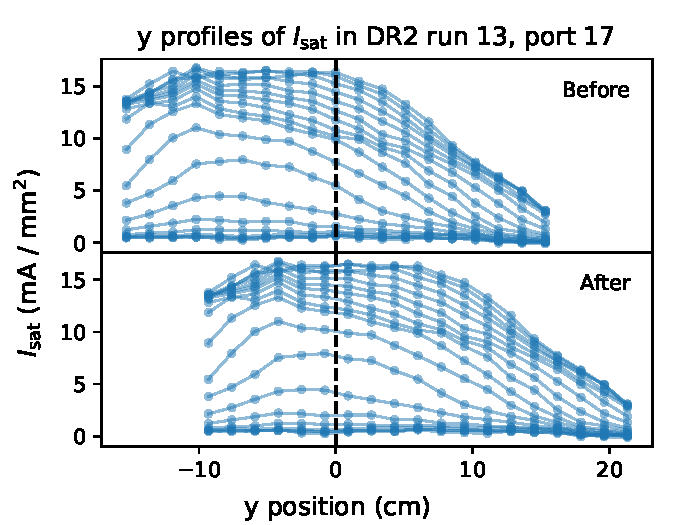
\includegraphics[width=300pt]{figures/y-alignment_before-after.pdf}
	\caption[y-axis profile before and after shifting the y-coordinate]{\label{fig:y-alignment_before-after}An example of the y-axis profile before and after shifting the y-coordinate. The ``before'' plot (top) is obviously asymmetrical about y=0. The shift needed to center was eyeballed from the plot. Each line represents a different x position, from closest to the core (upper lines) to the edge (lower lines).}
\end{figure}

\section{Applying and improving the dataset}

The two chapters following this detail machine learning studies utilizing this dataset, though only using a subset of the diagnostics available. Significant opportunities remain for ML-based analysis of the dataset, such as including additional diagnostics, in-situ diagnostic calibration (e.g., $I_\text{sat}$ or Thomson scattering). Even though the diversity of the dataset is relatively high, many imbalances in machine inputs remain. More data with additional (pseudo-)random samples from broader parameter ranges would be very beneficial in improving downstream ML tasks. Pushing the boundaries of the machine parameters could also lead to discovery and exploitation of new operational modes of the LAPD which could prove beneficial.

